\documentclass[12pt]{article}

\usepackage{sbc-template}
\usepackage{graphicx,url}
\usepackage[utf8]{inputenc}
\usepackage[brazil]{babel}
\usepackage{booktabs}
\usepackage{placeins}
\setlength{\textfloatsep}{8pt plus 2pt minus 4pt}
\setlength{\floatsep}{8pt plus 2pt minus 4pt}
\setlength{\intextsep}{8pt plus 2pt minus 4pt}
\usepackage{tikz}
\usetikzlibrary{arrows.meta}
\newcommand{\circled}[1]{\textcircled{\raisebox{-0.5pt}{\small #1}}}
\tolerance=9999
\emergencystretch=3em

\sloppy

\title{Ceres Diagnóstico: Sistema TinyML Embarcado para Detecção de
Doenças em Tomateiro com Validação Lab-Campo em Três Datasets}

\author{Namem Rachid Jaudy Neto\inst{1}}

\address{Instituto Federal de Educação, Ciência e Tecnologia de Mato Grosso (IFMT)\\
  Campus Cuiabá -- Cuiabá, MT -- Brasil
  \email{namem.rachid.jaudy@gmail.com}
}

\begin{document}
\maketitle

\begin{abstract}
This paper presents Ceres Diagnóstico, a low-cost embedded system for early
detection of tomato leaf diseases integrating TinyML, IoT, and a mobile application.
A MobileNetV2 INT8 model (638~KB), trained on PlantVillage (88{,}949 augmented
images) via two-phase transfer learning, is deployed across three inference
architectures:
ESP32-S3 edge (692~ms, offline), Android on-device via \texttt{tflite\_flutter}
($\approx$200--400~ms, offline), and Django REST API (306~ms, cloud). Five training
experiments document the impact of INT8 calibration (+34~pp over the uncalibrated
model; 2.37~pp residual loss vs.\ float), synthetic background augmentation
(ineffective), and real-data fine-tuning (+10~pp). The final model achieves 98.43\%
(float) on PlantVillage and 18--30\% on three independent field datasets,
quantifying the persistent lab-field gap.
\end{abstract}

\begin{resumo}
Este artigo apresenta o Ceres Diagnóstico, sistema embarcado de baixo custo para
detecção precoce de doenças foliares em tomateiro integrando TinyML, IoT e
aplicativo móvel. Um modelo MobileNetV2 INT8 (638~KB), treinado no PlantVillage
(88.949 imagens com \textit{augmentation}) via \textit{transfer learning} em duas
fases, é implantado em três arquiteturas de inferência: ESP32-S3 embarcado
(692~ms, offline), on-device no
Android via \texttt{tflite\_flutter} ($\approx$200--400~ms, offline) e API Django
REST (306~ms, nuvem). Cinco experimentos documentam o impacto da calibração INT8
(+34~pp sobre o modelo não-calibrado; 2,37~pp de perda residual vs.\ float),
augmentation sintética (ineficaz) e fine-tuning real (+10~pp). O modelo final atinge
98,43\% (float) no PlantVillage e 18--30\% em três datasets de campo,
quantificando o gap laboratório-campo.
\end{resumo}


%% ----------------------------------------------------------------
\section{Introdução}
%% ----------------------------------------------------------------

O tomateiro (\textit{Solanum lycopersicum}) é uma das culturas de maior importância
econômica no Brasil, com produção anual superior a 4 milhões de toneladas
\cite{fao2024}. Doenças foliares como requeima (\textit{Phytophthora infestans}),
septoriose (\textit{Septoria lycopersici}) e mancha-bacteriana (\textit{Xanthomonas}
spp.) podem causar perdas de até 100\% da safra \cite{embrapa2023}. O diagnóstico
tradicional depende de agrônomos especializados, inacessíveis à maioria dos pequenos
produtores rurais brasileiros.

Mohanty et al.~\cite{mohanty2016} demonstraram 99,35\% de acurácia no PlantVillage
em condições controladas, mas estudos subsequentes revelaram queda severa em campo
real: Singh et al.~\cite{singh2020} documentaram $\approx$31\% sem adaptação de
domínio; Xu et al.~\cite{xu2024} relataram quedas de até 58~pp ao transferir modelos
laboratoriais para campo.

Sistemas TinyML (\textit{Tiny Machine Learning}) permitem inferência de redes
neurais em microcontroladores sem dependência de nuvem \cite{warden2019} --- crítico
para regiões com conectividade instável como o Centro-Oeste brasileiro. Trabalhos
existentes em TinyML para
agricultura cobrem 4--5 classes de doença, não integram \textit{pipeline} IoT
completo e não validam desempenho em \textit{datasets} de campo real independentes.

Este trabalho apresenta o \textbf{Ceres Diagnóstico}, que: (1)~cobre 10~classes de
doenças; (2)~executa inferência no ESP32-S3 em 692~ms com modelo de 638~KB;
(3)~implementa três arquiteturas de inferência complementares (ESP32-S3, Android
on-device e API cloud) sobre o mesmo modelo; (4)~valida quantitativamente o gap em
3~\textit{datasets} independentes; (5)~documenta cinco experimentos com resultados
negativos reprodutíveis (\textit{augmentation} sintética ineficaz) e positivos
(\textit{fine-tuning} real $+$10~pp). Código e modelos disponíveis em
\url{https://github.com/Namem/extensao2}.

O restante deste artigo está organizado em cinco seções, incluindo esta introdução.
A Seção~2 discute os trabalhos relacionados; a Seção~3 detalha a metodologia
(arquitetura, modelo, \textit{dataset} e experimentos); a Seção~4 apresenta e discute os
resultados; e a Seção~5 traz a conclusão e os trabalhos futuros.


%% ----------------------------------------------------------------
\section{Trabalhos Relacionados}
%% ----------------------------------------------------------------

Mohanty et al.~\cite{mohanty2016} estabeleceram o estado da arte inicial com 99,35\%
no PlantVillage, mas em condições de laboratório (fundo uniforme, iluminação
controlada). Singh et al.~\cite{singh2020} introduziram o PlantDoc
(2.569~imagens de campo real, 27~espécies) e documentaram queda para $\approx$31\%
sem adaptação de domínio. Neste trabalho utiliza-se o subconjunto de tomateiro
(1.353~imagens) para validação independente. A remoção manual do fundo das imagens PlantDoc elevou a acurácia de
29,73\% para 70,53\% ($+$40,8~pp) sem modificar o modelo~\cite{singh2020},
confirmando que o modelo aprendeu o fundo como \textit{feature} discriminativa, não as lesões.
Xu et al.~\cite{xu2024} revisaram 42~trabalhos e quantificaram o gap em 29--58~pp,
concluindo que a maioria dos modelos de doenças em plantas carece de validação
em condições de campo. Barbedo~\cite{barbedo2019} documentou especificidade
geográfica severa: modelos treinados em \textit{datasets} de uma região apresentam queda
significativa ao serem aplicados em variedades e condições climáticas diferentes.

Para TinyML embarcado, Howard et al.~\cite{howard2017} e Sandler
et al.~\cite{sandler2018} propuseram MobileNet e MobileNetV2, arquiteturas projetadas
para hardware com restrições de memória e energia, reduzindo parâmetros de 138M
(VGG16) para 0,5M (MobileNetV2 alpha$=0{,}35$) sem perda crítica de acurácia.
Jacob et al.~\cite{jacob2018} demonstraram que a quantização INT8 sem
\textit{representative\_dataset} causa degradação severa dos fatores de escala ---
resultado reproduzido experimentalmente neste trabalho (Exp.~A: $-$30,5~pp).

O Ceres Diagnóstico se diferencia por: (a)~validação em 3~\textit{datasets} de campo
independentes em três continentes; (b)~\textit{pipeline} IoT completo, integrando
MQTT, API REST (\textit{Representational State Transfer}) e Flutter;
(c)~documentação de 5~experimentos com resultados negativos reprodutíveis.


%% ----------------------------------------------------------------
\section{Metodologia}
%% ----------------------------------------------------------------

Trata-se de uma pesquisa aplicada de natureza experimental, organizada em ciclos
iterativos de desenvolvimento e validação. O trabalho foi desenvolvido no Instituto
Federal de Mato Grosso (IFMT), Campus Cuiabá, no contexto de um Trabalho de
Conclusão de Curso, sem financiamento externo dedicado. A Tabela~\ref{tab:recursos}
sumariza os recursos de \textit{hardware} e \textit{software} empregados.

\begin{table}[ht]
\centering
\caption{Recursos de hardware e software utilizados.}
\label{tab:recursos}
\begin{tabular}{@{}lll@{}}
\toprule
\textbf{Etapa} & \textbf{Recurso} & \textbf{Versão / Especificação} \\
\midrule
Treinamento  & GPU NVIDIA RTX 3060 Ti           & 8~GB VRAM, CUDA (WSL2 Ubuntu) \\
Treinamento  & Python / TensorFlow              & 3.12 / 2.x \\
\textit{Backend} & Django REST + PostgreSQL      & Python 3.13 / PostgreSQL 18 \\
Embarcado    & ESP32-S3 N16R8                   & 240~MHz, PSRAM 8~MB \\
\textit{Firmware} & PlatformIO / ESP-IDF         & 5.x \\
Aplicativo   & Flutter / \texttt{tflite\_flutter} & 0.12.1 \\
Mensageria   & MQTT (HiveMQ / Mosquitto)        & TLS, porta 8883 \\
\bottomrule
\end{tabular}
\end{table}

O custo de \textit{hardware} do nó embarcado é de aproximadamente R\$~80 (ESP32-S3);
o treinamento utilizou GPU já disponível no laboratório e todo o \textit{software}
empregado é de código aberto ou gratuito, mantendo o custo total do projeto acessível
ao pequeno produtor rural.

\subsection{Arquitetura do Sistema}

O sistema implementa \textbf{três caminhos de inferência complementares} sobre o
mesmo modelo TFLite INT8 (638~KB), ilustrados na Figura~\ref{fig:arquitetura}:

\textbf{(1) Caminho Edge (ESP32-S3):} o modelo é executado diretamente no
microcontrolador ESP32-S3~N16R8 (240~MHz, PSRAM~8~MB) via TensorFlow Lite Micro,
sem qualquer dependência de rede para a inferência. O resultado (classe + confiança)
é publicado via MQTT sobre TLS (\textit{Transport Layer Security}) ao \textit{broker}
HiveMQ Cloud. A imagem \textbf{nunca sai do dispositivo}, garantindo privacidade por
design, em conformidade com a Lei Geral de Proteção de Dados (LGPD). Este caminho
foi validado
para inferência com benchmark de 10~imagens (latência 692~ms ±1~ms); a integração
da câmera OV5640 constitui etapa futura.

\textbf{(2) Caminho Mobile on-device (Flutter + \texttt{tflite\_flutter}):} o mesmo
modelo é carregado como asset no APK (\texttt{assets/models/ceres\_mobilenetv2\_int8.tflite})
e executado localmente no Android via \texttt{tflite\_flutter~0.12.1}, sem servidor.
Latência estimada de 200--400~ms, funciona \textit{offline}. Calibração de confiança
idêntica à do \textit{backend}: temperature scaling $T=0{,}25$ aplicado sobre os
logits antes do softmax.
O usuário alterna entre modo Local e modo Cloud diretamente na tela de câmera.

\textbf{(3) Caminho Cloud (Flutter + Django):} o aplicativo Flutter captura a
imagem com a câmera do \textit{smartphone}, envia via HTTPS à API Django (Railway),
que executa o mesmo modelo TFLite via Python \textit{subprocess} e retorna o
diagnóstico em JSON.
Este é o \textbf{sistema primário em produção}: \textit{pipeline} completo câmera~→~app~→~API~→~modelo~→~resultado validado \textit{end-to-end}. O \textit{backend} persiste o evento no
PostgreSQL e o app exibe histórico com \textit{cache} local (Drift/SQLite).

\begin{figure}[ht]
\centering
\begin{tikzpicture}[
  arr/.style={-{Stealth[length=2.5mm]}, thick, gray!80},
  ebox/.style={draw=blue!50,  fill=blue!7,         rounded corners=4pt,
               text width=2.8cm, minimum height=1.1cm, align=center, font=\footnotesize},
  abox/.style={draw=green!60!black, fill=green!7,  rounded corners=4pt,
               text width=2.8cm, minimum height=1.1cm, align=center, font=\footnotesize},
  cbox/.style={draw=purple!60,fill=purple!7,        rounded corners=4pt,
               text width=2.8cm, minimum height=1.1cm, align=center, font=\footnotesize},
  mbox/.style={draw=black!30, fill=black!6,         rounded corners=4pt,
               text width=9.6cm, minimum height=0.7cm, align=center,
               font=\footnotesize\bfseries},
  rebox/.style={draw=blue!50,  fill=blue!7,         rounded corners=4pt,
                text width=2.8cm, minimum height=0.8cm, align=center, font=\footnotesize},
  rabox/.style={draw=green!60!black, fill=green!7,  rounded corners=4pt,
                text width=2.8cm, minimum height=0.8cm, align=center, font=\footnotesize},
  rcbox/.style={draw=purple!60,fill=purple!7,        rounded corners=4pt,
                text width=2.8cm, minimum height=0.8cm, align=center, font=\footnotesize},
]
%% --- Linha 1: entradas ---
\node[ebox] (n1) at (0,   0) {\textbf{\circled{1} Edge}\\[3pt]
                               ESP32-S3 N16R8\\{\tiny 240\,MHz $\cdot$ PSRAM 8\,MB}};
\node[abox] (n2) at (3.8, 0) {\textbf{\circled{2} Mobile}\\[3pt]
                               Android\\{\tiny tflite\_flutter 0.12.1}};
\node[cbox] (n3) at (7.6, 0) {\textbf{\circled{3} Cloud}\\[3pt]
                               Flutter + Django\\{\tiny Railway $\cdot$ HTTPS}};
%% --- Linha 2: modelo compartilhado ---
\node[mbox] (model) at (3.8,-2.2)
  {MobileNetV2 INT8 $\cdot$ 638\,KB $\cdot$ $96{\times}96{\times}3$
   $\cdot$ 10 classes $\cdot$ $T{=}0{,}25$};
%% --- Linha 3: resultados ---
\node[rebox] (r1) at (0,   -3.9) {692\,ms $\pm$1\,ms\\{\tiny offline $\cdot$ MQTT/TLS}};
\node[rabox] (r2) at (3.8, -3.9) {$\approx$200--400\,ms\\{\tiny offline $\cdot$ toggle UI}};
\node[rcbox] (r3) at (7.6, -3.9) {306\,ms\\{\tiny cloud $\cdot$ PostgreSQL}};
%% --- Setas entrada → modelo ---
\draw[arr, blue!70]        (n1.south) -- ++(0,-0.35)
    -| ([xshift=-3.8cm]model.north);
\draw[arr, green!60!black] (n2.south) -- (model.north);
\draw[arr, purple!70]      (n3.south) -- ++(0,-0.35)
    -| ([xshift=3.8cm]model.north);
%% --- Setas modelo → resultados ---
\draw[arr] ([xshift=-3.8cm]model.south) |- (r1.north);
\draw[arr] (model.south) -- (r2.north);
\draw[arr] ([xshift= 3.8cm]model.south) |- (r3.north);
\end{tikzpicture}
\caption{Três caminhos de inferência sobre o mesmo modelo MobileNetV2 INT8 (638\,KB).
         \textbf{\circled{1}~Edge:} TFLite Micro no ESP32-S3, imagens embarcadas
         como arrays~C (latência CNN pura, sem sensor).
         \textbf{\circled{2}~Mobile:} \texttt{tflite\_flutter} on-device no Android,
         offline total.
         \textbf{\circled{3}~Cloud:} API Django (Railway), Python subprocess TFLite.}
\label{fig:arquitetura}
\end{figure}

\subsection{Modelo MobileNetV2 INT8}

\textbf{Arquitetura:} MobileNetV2 \cite{sandler2018} alpha$=0{,}35$, entrada
96$\times$96$\times$3~RGB, backbone pré-treinado ImageNet, cabeça:
GlobalAveragePooling~+ Dropout(0,3)~+ Dense(10,~softmax).

\textbf{Treinamento em duas fases:} Fase~1 (10~épocas, LR$=1\!\times\!10^{-3}$) ---
backbone congelado, apenas a cabeça treinada; val\_acc estabiliza em 87,4\%.
Fase~2 (40~épocas, LR$=5\!\times\!10^{-4}$) --- últimas 30~camadas descongeladas,
EarlyStopping($p=8$) + ReduceLROnPlateau($f=0{,}5$). A melhor acurácia de validação
(97,90\%) ocorre na época~46, como ilustra a Figura~\ref{fig:treino}.

\begin{figure}[ht]
\centering
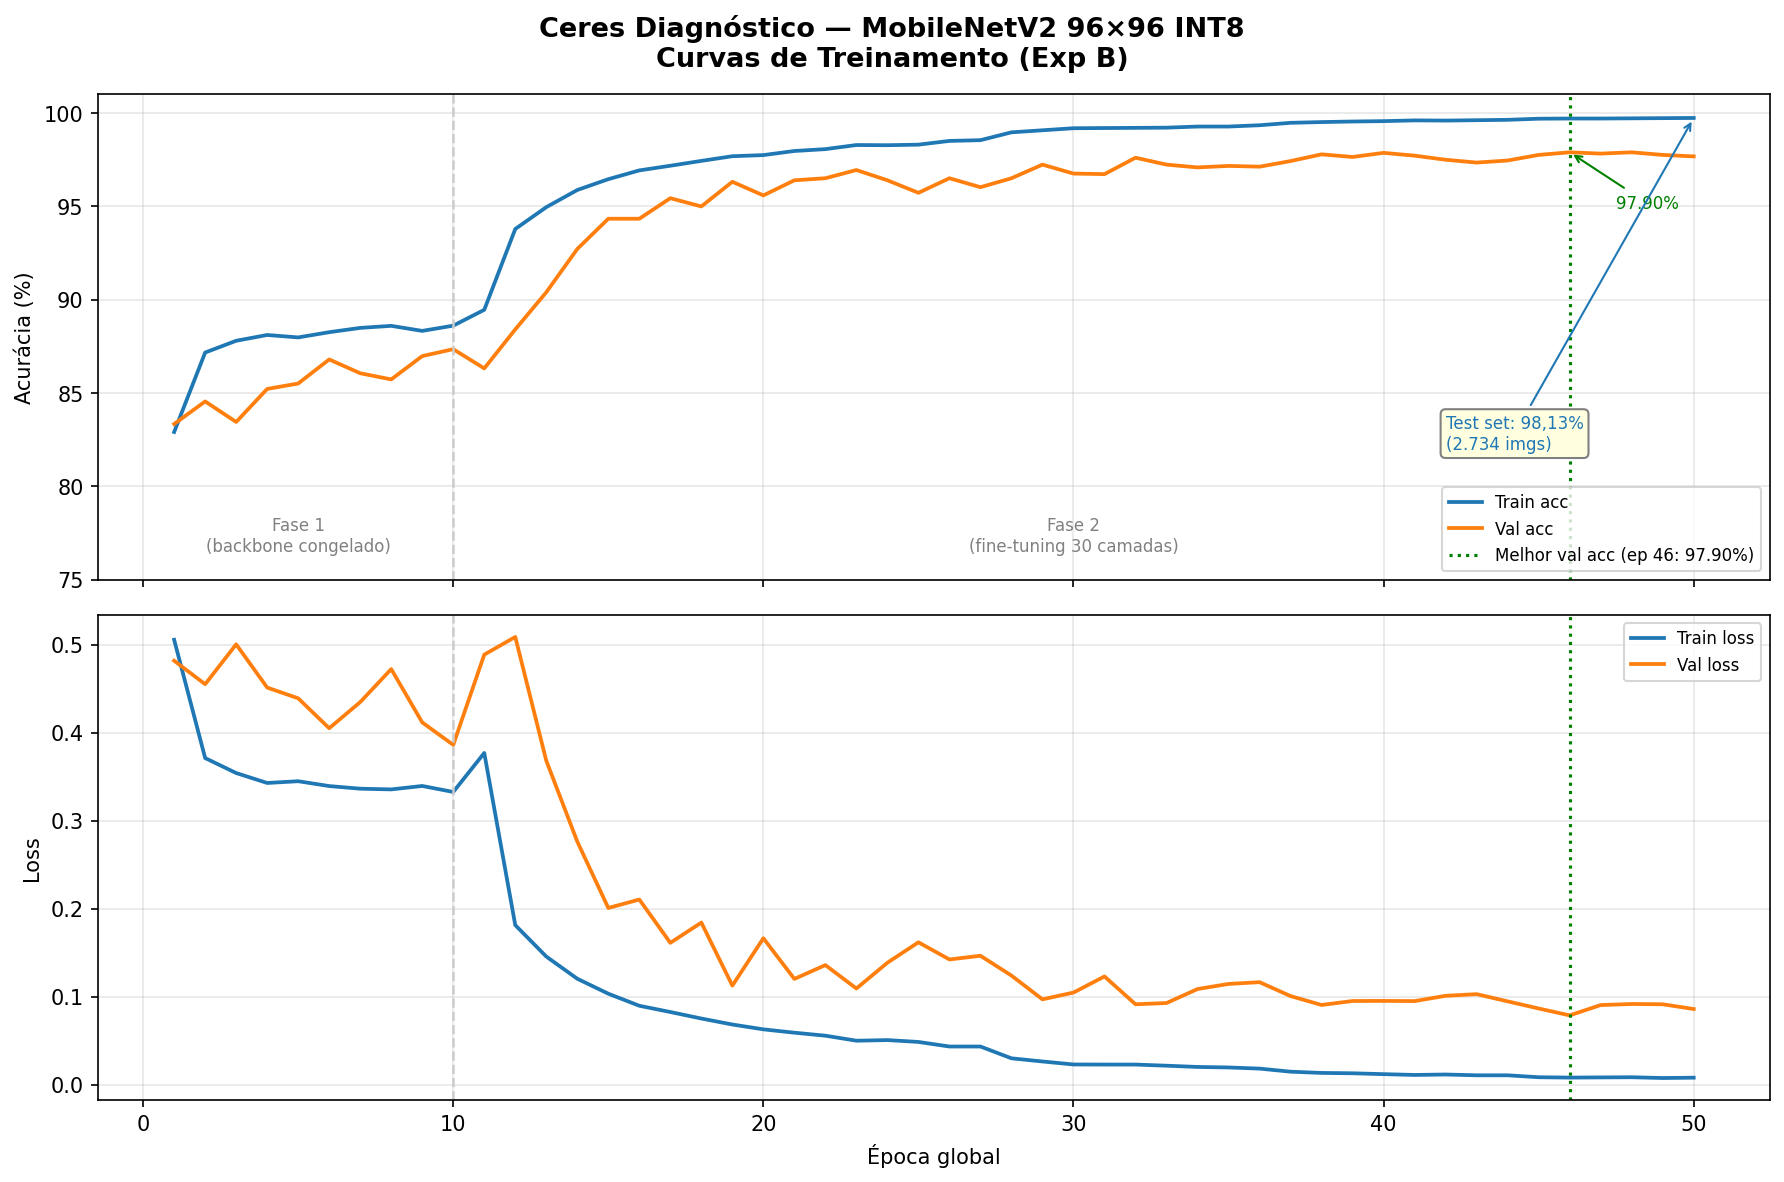
\includegraphics[width=0.92\textwidth]{historico_treino.png}
\caption{Curvas de treinamento do Exp.~B (MobileNetV2 96$\times$96). A linha vertical
tracejada marca a transição da Fase~1 (\textit{backbone} congelado) para a Fase~2
(\textit{fine-tuning} das últimas 30~camadas). A melhor acurácia de validação
(97,90\%, época~46) corresponde a 98,13\% no \textit{test set} para o modelo float.}
\label{fig:treino}
\end{figure}

\textbf{Quantização INT8 calibrada:} 50~batches do \textit{val set} como
\textit{representative\_dataset} \cite{jacob2018}. Sem calibração, a quantização
degrada a acurácia em $-$30,5~pp (Exp.~A); com calibração, a perda residual cai para
apenas 2,37~pp (98,13\% float $\to$ 95,76\% INT8 no \textit{test set}).
\textbf{Pós-processamento:} temperature scaling ($T=0{,}25$) aplicado ao vetor de
logits antes do softmax em todos os caminhos de inferência (ESP32-S3, Android
on-device e Django), calibrando a confiança reportada ao usuário.

\subsection{Dataset}

\textbf{PlantVillage} \cite{hughes2015}: 18.160~imagens, 10~classes, CC~BY~4.0.
\textit{Split} estratificado (seed$=42$): 70\% treino / 15\% val / 15\% teste.
\textit{Augmentation} \textit{offline} (só treino): \textit{flip} H/V, rotação $\pm$15°, brilho $\pm$20\%.
Resultado: 88.949~imagens de treino.

\textbf{Datasets de campo real} (validação independente):
PlantDoc \cite{singh2020} --- 1.353~imagens (EUA/Europa);
Tomato-Village \cite{gehlot2023} --- 217~imagens (Rajastão, Índia, 2022);
Daffodil~BD~\cite{daffodilbd2024} --- 1.616~imagens (Bangladesh).

\subsection{Experimentos}

Cinco experimentos documentam a evolução do modelo (Tabela~\ref{tab:experimentos}).

\begin{table}[ht]
\centering
\caption{Configuração dos cinco experimentos de treinamento.}
\label{tab:experimentos}
\begin{tabular}{@{}llp{5.5cm}@{}}
\toprule
\textbf{Exp.} & \textbf{Plataforma} & \textbf{Estratégia principal} \\
\midrule
A & Edge Impulse (nuvem) & Sem calibração INT8 \\
B & TF local WSL2 & 2 fases + calibração INT8 (50 batches) \\
C & TF local WSL2 & Exp.~B + background aug.\ sintética (rembg U2-Net) \\
D & TF local WSL2 & Exp.~B + fine-tuning com PlantDoc/train real \\
E & TF local WSL2 & Exp.~D + Focal Loss ($\gamma=2$) + aug.\ agressiva \\
\bottomrule
\end{tabular}
\end{table}

\subsection{Experimento Edge vs.\ Cloud}

Mesmo modelo TFLite INT8 (Exp.~E, 638~KB) executado em três ambientes:
\textbf{Edge} --- ESP32-S3~N16R8, 240~MHz, latência medida com
\texttt{esp\_timer\_get\_time()}; \textbf{Mobile} --- Android, latência estimada
via \texttt{tflite\_flutter} (não medida empiricamente neste ciclo);
\textbf{Cloud} --- Django REST (Railway), Python subprocess TFLite, servidor Linux.

\subsection{Firmware e Pipeline IoT}

Firmware PlatformIO/ESP-IDF~5.x: modelo carregado como array~C no flash, arena de
inferência em PSRAM (200~KB de 512~KB alocados). A opção por imagens pré-carregadas
como arrays~C --- em vez da câmera OV5640 --- foi deliberada para isolar a latência
da CNN pura da latência de captura do sensor, garantindo medição comparável à
literatura. A câmera constitui etapa futura de integração. Resultado publicado via
MQTT com QoS~1 (\textit{Quality of Service}, TLS) ao \textit{broker} HiveMQ Cloud
(porta~8883); \textit{broker} Mosquitto local utilizado apenas em desenvolvimento.
O \textit{backend} Django persiste o evento em PostgreSQL e expõe o histórico via
REST. O aplicativo Flutter captura a coordenada GPS (\textit{Global Positioning
System}) do dispositivo antes de cada inferência e a inclui no POST de diagnóstico.
O \textit{cache} local é gerenciado pelo Drift (SQLite) com \texttt{SyncService}, que
reenvia automaticamente diagnósticos pendentes ao restaurar conectividade
(\textit{offline-first}).

\subsection{Justificativa das Tecnologias Principais}

\textbf{MobileNetV2 vs.\ alternativas:} A escolha da arquitetura foi determinada
pela restrição de memória do ESP32-S3 ($<$4~MB RAM utilizável para o modelo).
A Tabela~\ref{tab:modelos} compara as principais alternativas de Redes Neurais
Convolucionais (CNN) consideradas.

\begin{table}[ht]
\centering
\caption{Comparativo de arquiteturas CNN para implantação no ESP32-S3.}
\label{tab:modelos}
\begin{tabular}{@{}lrrc@{}}
\toprule
\textbf{Modelo} & \textbf{Parâmetros} & \textbf{RAM} & \textbf{ESP32-S3?} \\
\midrule
VGG16          & 138M  & $>$500~MB & Não \\
ResNet-50      & 25M   & $>$100~MB & Não \\
EfficientNet-B0 & 5,3M & $\approx$20~MB & Não \\
YOLO (mínimo)  & $\approx$6M & $>$10~MB & Não* \\
MobileNetV1    & 4,2M  & $\approx$3~MB & Sim (inferior) \\
\textbf{MobileNetV2} & \textbf{3,4M} & \textbf{$<$4~MB} & \textbf{Sim} \\
\bottomrule
\multicolumn{4}{l}{\footnotesize *YOLO: detector de objetos (bounding box), incompatível com classificação de folha.}
\end{tabular}
\end{table}

Além do tamanho, o MobileNetV2 usa \textit{depthwise separable convolutions} e
\textit{inverted residuals com linear bottleneck}~\cite{sandler2018}, reduzindo
FLOPs sem perda crítica de acurácia. O alpha$=0{,}35$ reduz parâmetros para 0,5M,
gerando modelo INT8 de 638~KB.

\textbf{ESP32-S3 vs.\ Raspberry Pi~4:} O ESP32-S3~N16R8 foi escolhido por custo
($\approx$R\$~80 vs.\ R\$~400$+$ do RPi~4), ausência de sistema operacional
(menor superfície de ataque, boot instantâneo), consumo ($<$500~mW vs.\ $>$5~W)
e suporte nativo ao TFLite Micro \cite{warden2019}. O Raspberry Pi seria viável
para modelos maiores (EfficientNet-B0), mas inviável para \textit{deploy} rural de baixo custo.

\textbf{MQTT vs.\ HTTP:} O MQTT opera com header de apenas 2~bytes e suporta
QoS~0/1/2, projetado para redes instáveis e microcontroladores (MCUs) com recursos
limitados. O HTTP
REST exige header de $\approx$800~bytes e não oferece QoS nativo --- inadequado
para comunicação ESP32~→~servidor em ambiente rural \cite{oasis2019}.


%% ----------------------------------------------------------------
\section{Resultados e Discussão}
%% ----------------------------------------------------------------

\subsection{Impacto da Calibração INT8 (Exp.~A vs.\ Exp.~B)}

\begin{table}[ht]
\centering
\caption{Comparativo Exp.~A (Edge Impulse) vs.\ Exp.~B (TensorFlow local).
O modelo efetivamente embarcado no ESP32-S3 é o INT8.}
\label{tab:ab}
\begin{tabular}{@{}lrrrr@{}}
\toprule
\textbf{Métrica} & \textbf{Exp.~A FP32} & \textbf{Exp.~A INT8} & \textbf{Exp.~B float} & \textbf{Exp.~B INT8} \\
\midrule
Acurácia val set  & 92,5\% & 62,0\% & 97,90\% & --- \\
Acurácia test set & ---    & ---    & 98,13\% & \textbf{95,76\%} \\
Macro F1          & 0,92   & 0,62   & 0,977   & --- \\
Tamanho modelo    & 1.637~KB & 547~KB & ---    & \textbf{638~KB} \\
\bottomrule
\end{tabular}
\end{table}

A ausência de \textit{representative\_dataset} no Exp.~A causou queda de 30,5~pp
(92,5\%~$\to$~62,0\%), confirmando Jacob et al.~\cite{jacob2018}. As classes mais
afetadas foram D01\_requeima ($-$30,7~pp) e D03b\_mancha\_alvo ($-$28,6~pp) ---
as com menos amostras no \textit{val set}, evidenciando que a representatividade do
\textit{dataset} de calibração determina diretamente a qualidade dos fatores de
escala (scale e zero-point) por tensor.

O Exp.~B, com calibração sobre 50~batches reais do \textit{val set}, reduz a perda de
quantização a apenas 2,37~pp: o modelo float atinge 98,13\% e o INT8 embarcado,
95,76\% no \textit{test set} (Figura~\ref{fig:matriz}) --- ainda assim $+$33,8~pp
acima do INT8 não-calibrado do Exp.~A (62,0\%). A calibração adequada, portanto,
não elimina totalmente a perda, mas a torna desprezível para a aplicação.

\begin{figure}[ht]
\centering
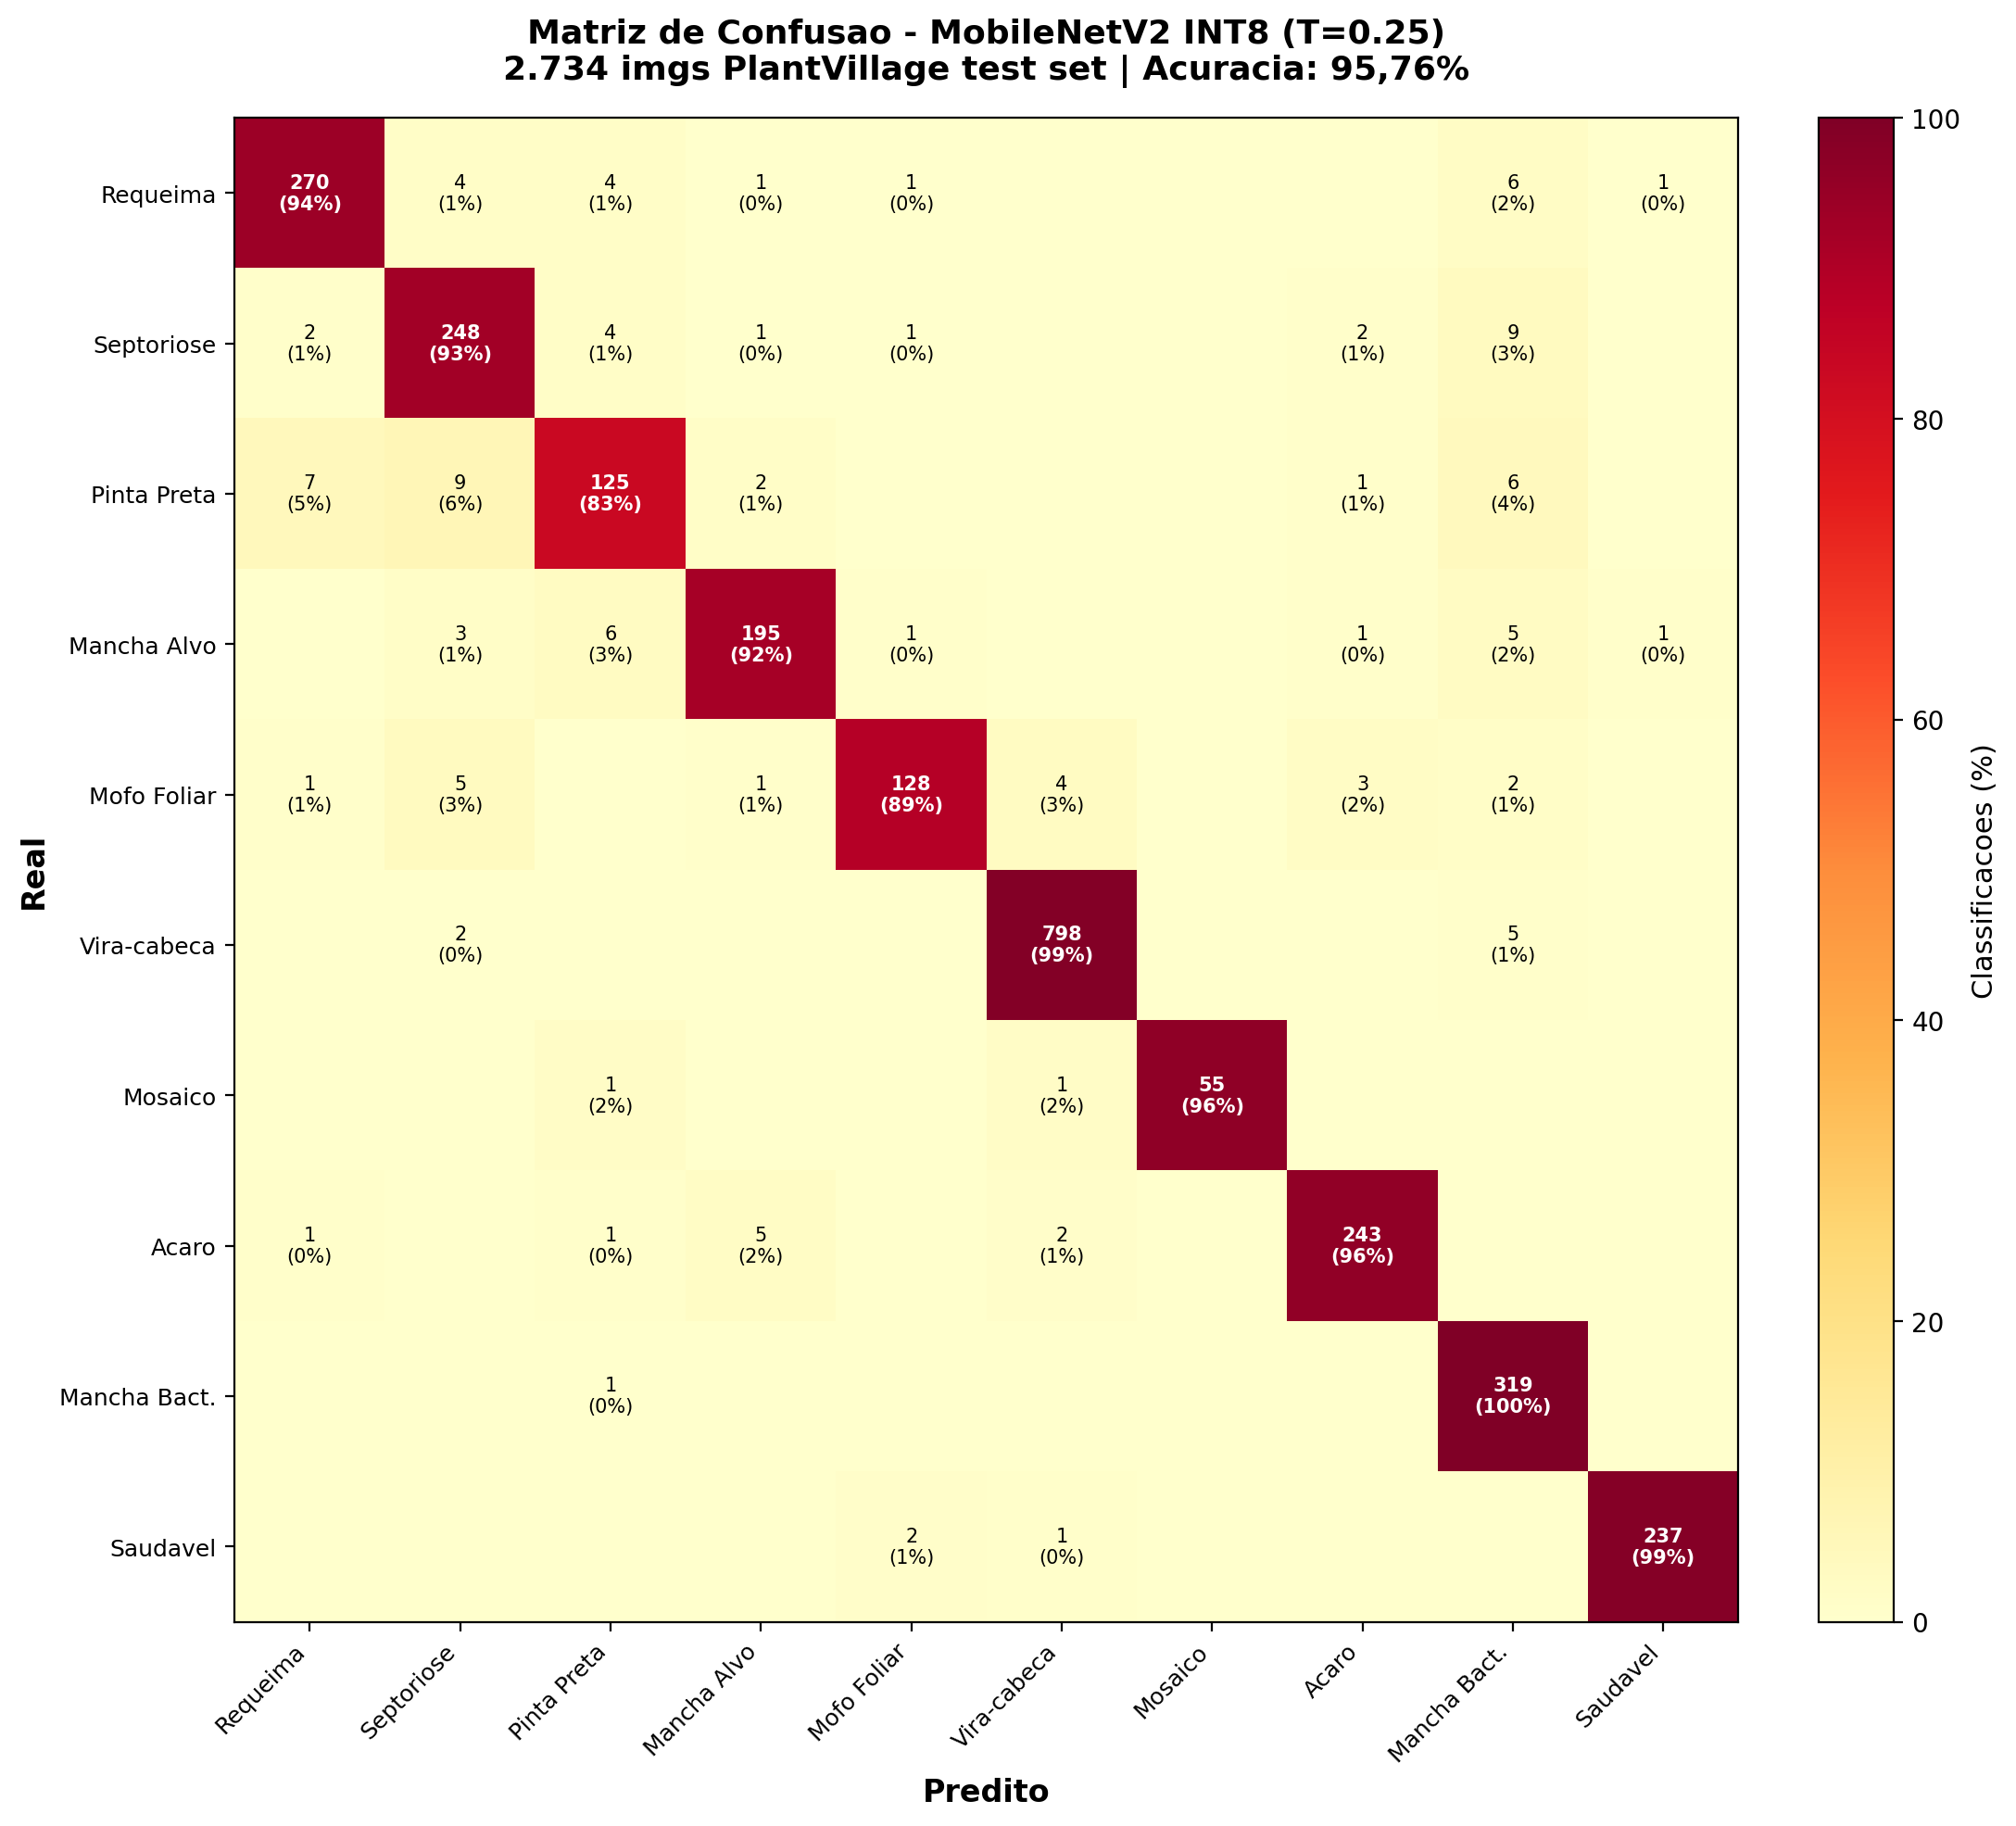
\includegraphics[width=0.78\textwidth]{matriz_confusao_int8.png}
\caption{Matriz de confusão do modelo INT8 ($T=0{,}25$) no \textit{test set} do
PlantVillage (2.734~imagens, acurácia 95,76\%). As maiores confusões ocorrem entre
pinta-preta, septoriose e requeima --- doenças com lesões necróticas visualmente
semelhantes.}
\label{fig:matriz}
\end{figure}

\FloatBarrier
\subsection{Latência no ESP32-S3}

A latência medida foi de \textbf{692~ms} (desvio padrão $\pm$1~ms, determinístico),
com 10/10~imagens corretas no benchmark. A arena PSRAM ocupa 200~KB de 512~KB
alocados (39\%), deixando margem para modelos maiores. A latência real (692~ms)
ficou cerca de 2$\times$ abaixo da estimativa do Edge Impulse (1.365~ms), indicando
que simuladores tendem a superestimar o tempo de inferência do Xtensa~LX7 em
operações INT8.

A meta de 300~ms não foi atingida. O fator limitante é a ausência de unidade SIMD
(\textit{Single Instruction, Multiple Data}) INT8 dedicada no Xtensa~LX7 --- as
operações de convolução são executadas via
instruções escalares de propósito geral, sem aceleração vetorial. Contudo, 692~ms
é imperceptível no contexto agrícola: o tempo humano para posicionar e estabilizar
a folha diante da câmera é da ordem de 2--5~segundos. A variância determinística
($\pm$1~ms) garante previsibilidade total, independente de condições de rede.

\subsection{Gap Laboratório-Campo}

\begin{table}[ht]
\centering
\caption{Acurácia por experimento em lab e campo (três datasets independentes).}
\label{tab:gap}
\begin{tabular}{@{}lcccc@{}}
\toprule
\textbf{Exp.} & \textbf{PlantVillage} & \textbf{PlantDoc} & \textbf{Tomato-Village} & \textbf{Daffodil~BD} \\
              & \textbf{(test, lab)}  & \textbf{(campo)}  & \textbf{(campo)}        & \textbf{(campo)} \\
\midrule
B -- baseline      & 98,13\% & 20,77\% & --- & --- \\
C -- aug.\ sintét. & 96,20\% & 20,24\% & --- & --- \\
D -- fine-tun.\ real & 97,55\% & \textbf{30,43\%} & 11,52\% & --- \\
E -- Focal Loss    & \textbf{98,43\%} & 30,43\% & \textbf{27,65\%} & \textbf{18,13\%} \\
\bottomrule
\multicolumn{5}{p{0.95\linewidth}}{\footnotesize Coluna lab: acurácia do modelo
float no \textit{test set}; o INT8 embarcado do Exp.~B atinge 95,76\%
(Fig.~\ref{fig:matriz}). Colunas de campo: modelo INT8 (mesma quantização do ESP32-S3).}
\end{tabular}
\end{table}

Tomato-Village e Daffodil~BD foram avaliados apenas nos modelos finais (Exp.~D e~E),
como teste adicional de generalização geográfica; os experimentos B e~C, anteriores,
não foram reexecutados sobre eles --- daí as células~``---'' na Tabela~\ref{tab:gap}.

\textbf{\textit{Background augmentation} sintética (Exp.~C):} Remoção de fundo com rembg
U2-Net~\cite{qin2020} e recomposição sobre fundos PlantDoc não melhorou o
desempenho de campo ($+$0~pp vs.\ Exp.~B). Artefatos de borda e inconsistências de
iluminação nas composições sintéticas impedem a transferência para o domínio real
\cite{ganin2016}. O caso mais revelador foi a classe \texttt{saudavel}: mesmo após
177.698~composições sintéticas, o modelo nunca prediz folha saudável em campo
(0,0\%), indicando que o domínio sintético não captura a distribuição real dessas
imagens. Este é um resultado negativo reprodutível, documentado segundo as
diretrizes de Pineau et al.~\cite{pineau2021}.

\textbf{\textit{Fine-tuning} com dados reais (Exp.~D):} Adição de 677~imagens do
PlantDoc/train (repetidas 10$\times$) produziu ganho real de $+$10~pp
(20,77\%~$\to$~30,43\%) em 69~imagens nunca vistas. O fator limitante é o
\textbf{volume de dados de campo}, não o método de treinamento.

\textbf{Focal Loss (Exp.~E):} Focal Loss ($\gamma=2$)~\cite{lin2017} melhorou
consistência entre \textit{datasets} (+16~pp no Tomato-Village: 11,52\%~$\to$~27,65\%).
O mecanismo é a redução de peso para exemplos fáceis (imagens laboratoriais com
fundo cinza), forçando o modelo a focar nas \textit{features} diagnósticas da lesão.

\textbf{Gap geográfico:} A acurácia cai com a distância geográfica do PlantDoc:
EUA/Europa (30,43\%) $>$ Índia (27,65\%) $>$ Bangladesh (18,13\%), confirmando
Barbedo~\cite{barbedo2019}: modelos PlantVillage exibem especificidade geográfica
em função de variedades locais, condições de iluminação tropical e estágio
fenológico distinto.

\textbf{Colapso de classe:} No Exp.~D avaliado no Tomato-Village, o modelo
classificou D02\_septoriose para 73\% das folhas saudáveis indianas --- padrão de
colapso sob shift de domínio extremo. Parcialmente mitigado no Exp.~E com Focal Loss.

\subsection{Edge vs.\ Cloud}

\begin{table}[ht]
\centering
\caption{Comparativo Edge (ESP32-S3) vs.\ Cloud (Django REST).}
\label{tab:edge}
\begin{tabular}{@{}lccc@{}}
\toprule
\textbf{Aspecto} & \textbf{Edge -- ESP32-S3} & \textbf{Mobile -- Android} & \textbf{Cloud -- Django} \\
\midrule
Latência inferência    & 692~ms ($\pm$1~ms) & $\approx$200--400~ms & 306~ms (subprocess) \\
Latência end-to-end    & 692~ms             & $\approx$200--400~ms & 2.333~ms (HTTP dev) \\
Funciona offline       & \textbf{Sim}       & \textbf{Sim}         & Não \\
Privacidade (LGPD)     & \textbf{Total}     & \textbf{Total}       & Imagem transmitida \\
Custo adicional        & $\approx$R\$~80    & Zero (app)           & Servidor PC/cloud \\
\bottomrule
\end{tabular}
\end{table}

O ESP32-S3 é superior para zonas rurais sem conectividade estável e para cenários
de privacidade (LGPD), já que a imagem nunca sai do dispositivo. A latência Cloud
de 2.333~ms reflete o servidor de desenvolvimento Django (\textit{single-thread},
Windows); estima-se que em produção com Gunicorn \textit{multi-worker} e modelo
\textit{singleton} em memória, a latência HTTP seria $<$200~ms \textit{end-to-end}
--- ainda assim superior ao ESP32-S3 para o caso \textit{offline}, mas complementar
para produtores com conectividade estável.


%% ----------------------------------------------------------------
\section{Conclusão}
%% ----------------------------------------------------------------

O Ceres Diagnóstico demonstrou a viabilidade de um sistema TinyML completo
executando MobileNetV2 INT8 (638~KB) no ESP32-S3 com 692~ms de latência
determinística. As principais contribuições são:

\begin{enumerate}
  \item \textbf{Pipeline reproduzível:} PlantVillage $\to$ 88.949~imgs $\to$
        MobileNetV2 INT8 $\to$ ESP32-S3, código aberto (\url{https://github.com/Namem/extensao2}).
  \item \textbf{Quantificação da calibração INT8:} $+$34~pp com
        \textit{representative\_dataset} (62,0\%~$\to$~95,76\%) vs.\ quantização
        automática, com perda residual de apenas 2,37~pp frente ao modelo float.
  \item \textbf{Benchmark em 3 \textit{datasets} de campo independentes:} documentação do
        gap lab-campo (98,43\% $\to$ 18--30\%) e sua natureza geográfica.
  \item \textbf{Resultado negativo reprodutível:} \textit{background augmentation} sintética
        ineficaz; \textit{fine-tuning} com dados reais confirma volume como fator limitante.
  \item \textbf{Comparativo Edge, Mobile e Cloud:} latência do ESP32-S3 e do
        Django medida empiricamente em hardware real (Android on-device estimado).
\end{enumerate}

\textbf{Limitações:} A latência de 692~ms ficou acima da meta de 300~ms (hardware
sem acelerador INT8 dedicado). A câmera OV5640 não foi integrada neste ciclo ---
a validação usou imagens embutidas como arrays~C. O gap laboratório-campo
(98,43\% $\to$ 18--30\%) persiste como problema aberto: augmentation sintética
é insuficiente e dados de campo reais são escassos para o Brasil.

\textbf{Lições aprendidas:} a principal lição deste ciclo é que, no domínio
agrícola, o volume e a representatividade dos dados de campo pesam mais que a
sofisticação do método de treinamento --- o \textit{fine-tuning} com apenas
677~imagens reais (Exp.~D) superou a \textit{augmentation} sintética em larga escala
(Exp.~C, 177.698
composições). Além disso, a calibração INT8 com \textit{representative\_dataset}
mostrou-se determinante: um detalhe de implementação ($-$30,5~pp se omitido) com
impacto maior que mudanças de arquitetura.

Trabalhos futuros incluem coleta de \textit{dataset} em lavouras de Sorriso-MT para
\textit{fine-tuning} supervisionado com variedades locais, \textit{domain adaptation}
adversarial (DANN~\cite{ganin2016}) sem necessidade de \textit{labels} de campo,
integração da câmera
OV5640, e validação de usabilidade com produtores rurais.


%% ----------------------------------------------------------------
\section*{Uso de Inteligência Artificial Generativa}
%% ----------------------------------------------------------------

O autor declara que ferramentas de inteligência artificial generativa
foram utilizadas como auxílio na revisão gramatical, organização do
texto e formatação de seções deste artigo. Todo o conteúdo técnico,
experimentos, análises e conclusões são de autoria exclusiva do autor.

%% ----------------------------------------------------------------
\bibliographystyle{sbc}
\bibliography{referencias}
%% ----------------------------------------------------------------

\end{document}
